\section{Basic Concepts}

\begin{frame}{Supervised vs. Unsupervised Learning}
	\begin{itemize}
		\item \textbf{\color{airforceblue}Supervised learning (classification).}
		      \begin{itemize}
			      \item Supervision:
			            \begin{itemize}
				            \item The \textbf{training data} (observations, measurements, etc.) are accompanied by \textbf{labels} indicating the \textbf{class} of the observations.
				            \item New data is classified based on a \textbf{model} created from the training data.
			            \end{itemize}
		      \end{itemize}
		\item \textbf{\color{airforceblue}Unsupervised learning (clustering).}
		      \begin{itemize}
			      \item The class labels of training data are unknown.
			            \begin{itemize}
				            \item Or rather, there are no training data.
			            \end{itemize}
		      \end{itemize}
		      \begin{itemize}
			      \item Given a set of measurements, observations, etc., \\ the goal is to find classes or clusters in the data.
			            \begin{itemize}
				            \item See next chapter.
			            \end{itemize}
		      \end{itemize}
	\end{itemize}
\end{frame}

\begin{frame}{Prediction Problems: Classification vs. Numerical Prediction}
	\begin{itemize}
		\item \textbf{Classification:}
		      \begin{itemize}
			      \item Predicts \textbf{\color{airforceblue}categorical class labels} (discrete, nominal).
			      \item Constructs a model based on the training set and the values (class labels) in a classifying attribute and uses it in classifying new data.
		      \end{itemize}
		\item \textbf{Numerical prediction:}
		      \begin{itemize}
			      \item Models \textbf{\color{airforceblue}continuous-valued functions}.
			      \item I.e. predicts missing or unknown (future) values.
		      \end{itemize}
		\item \textbf{Typical applications of classification:}
		      \begin{itemize}
			      \item Credit/loan approval: Will it be paid back?
			      \item Medical diagnosis: Is a tumor cancerous or benign?
			      \item Fraud detection: Is a transaction fraudulent or not?
			      \item Web-page categorization: Which category is it?
		      \end{itemize}
	\end{itemize}
\end{frame}

\begin{frame}{Classification -- A Two-step Process}
	\begin{itemize}
		\item \textbf{Model construction: describing a set of predetermined classes:}
		      \begin{itemize}
			      \item Each tuple/sample is assumed to belong to a predefined class, as determined by the \textbf{\color{airforceblue}class-label attribute}.
			      \item The set of tuples used for model construction is the \textbf{\color{airforceblue}training set}.
			      \item The \textbf{\color{airforceblue}model} is represented as classification rules, decision trees, or mathematical formulae.
		      \end{itemize}
		\item \textbf{Model usage, for classifying future or unknown objects:}
		      \begin{itemize}
			      \item Estimate \textbf{\color{airforceblue}accuracy} of the model:
			            \begin{itemize}
				            \item The known label of \textbf{test samples} is compared with the result from the model.
				            \item \textbf{Accuracy rate} is the percentage of test-set samples that are correctly classified by the model.
				            \item Test set is independent of training set (otherwise overfitting).
			            \end{itemize}
			      \item If the accuracy is acceptable, \textbf{\color{airforceblue}use the model} to classify data tuples whose class labels are not known.
		      \end{itemize}
	\end{itemize}
\end{frame}

\begin{frame}{Classification -- A Two-step Process}
	\centering
	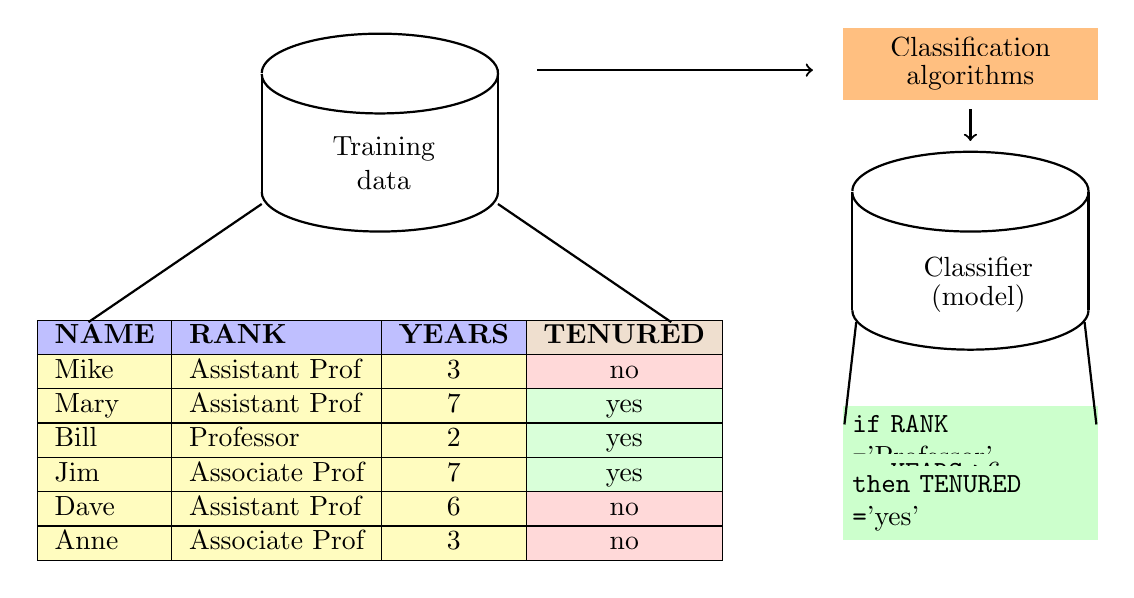
\begin{tikzpicture}
		\node at (0,0) {
			\begin{tabular}{|l|l|c|c|}
				\hline
				\cellcolor{blue!25}\textbf{\uppercase{name}} & \cellcolor{blue!25}\textbf{\uppercase{rank}} & \cellcolor{blue!25}\textbf{\uppercase{years}} & \cellcolor{brown!25}\textbf{\uppercase{tenured}} \\\hline
				\cellcolor{yellow!25}Mike                    & \cellcolor{yellow!25}Assistant Prof          & \cellcolor{yellow!25}3                        & \cellcolor{red!15}no                             \\\hline
				\cellcolor{yellow!25}Mary                    & \cellcolor{yellow!25}Assistant Prof          & \cellcolor{yellow!25}7                        & \cellcolor{green!15}yes                          \\\hline
				\cellcolor{yellow!25}Bill                    & \cellcolor{yellow!25}Professor               & \cellcolor{yellow!25}2                        & \cellcolor{green!15}yes                          \\\hline
				\cellcolor{yellow!25}Jim                     & \cellcolor{yellow!25}Associate Prof          & \cellcolor{yellow!25}7                        & \cellcolor{green!15}yes                          \\\hline
				\cellcolor{yellow!25}Dave                    & \cellcolor{yellow!25}Assistant Prof          & \cellcolor{yellow!25}6                        & \cellcolor{red!15}no                             \\\hline
				\cellcolor{yellow!25}Anne                    & \cellcolor{yellow!25}Associate Prof          & \cellcolor{yellow!25}3                        & \cellcolor{red!15}no                             \\\hline
			\end{tabular}
		};
		\node[fill=orange!50, text width = 3cm, align=center] at (7.5,5) {Classification};
		\node[fill=orange!50, text width = 3cm, align=center] at (7.5,4.6) {algorithms};

		\node[fill=green!20, text width = 3cm, align=left] at (7.5,0) {\texttt{if RANK =}'Professor'};
		\node[fill=green!20, text width = 3cm, align=left] at (7.5,-0.4) {\texttt{or YEARS >}6};
		\node[fill=green!20, text width = 3cm, align=left] at (7.5,-0.8) {\texttt{then TENURED =}'yes'};

		\node[text width = 3cm, align=center] at (0.05,3.7) {Training};
		\node[text width = 3cm, align=center] at (0.05,3.3) {data};

		\node[text width = 3cm, align=center] at (7.6,2.2) {Classifier};
		\node[text width = 3cm, align=center] at (7.6,1.8) {(model)};

		\draw [thick](-1.5,3.15) -- (-1.5,4.65);
		\draw [thick](1.5,3.15) -- (1.5,4.65);
		\draw [thick](-1.5,3.15) arc (180:360:1.5 and 0.5);
		\draw [thick](-1.5,4.65) arc (180:360:1.5 and 0.5);
		\draw [thick](1.5,4.65) arc (-1.5:180:1.5 and 0.5);
		\draw [thick, ->] (2,4.7) -- (5.5,4.7);
		\draw [thick, ->] (7.5,4.2) -- (7.5,3.8);
		\draw [thick] (6.05,1.5) -- (5.9,0.2);
		\draw [thick] (8.95,1.5) -- (9.1,0.2);

		\draw [thick](6,1.65) -- (6,3.15);
		\draw [thick](9,1.65) -- (9,3.15);
		\draw [thick](6,1.65) arc (180:360:1.5 and 0.5);
		\draw [thick](6,3.15) arc (180:360:1.5 and 0.5);
		\draw [thick](9,3.15) arc (-1.5:180:1.5 and 0.5);
		\draw [thick] (-3.7,1.5) -- (-1.5,3);
		\draw [thick] (1.5,3) -- (3.7,1.5);
	\end{tikzpicture}
\end{frame}

\begin{frame}{Process (II): Using the Model in Prediction}
	\centering
	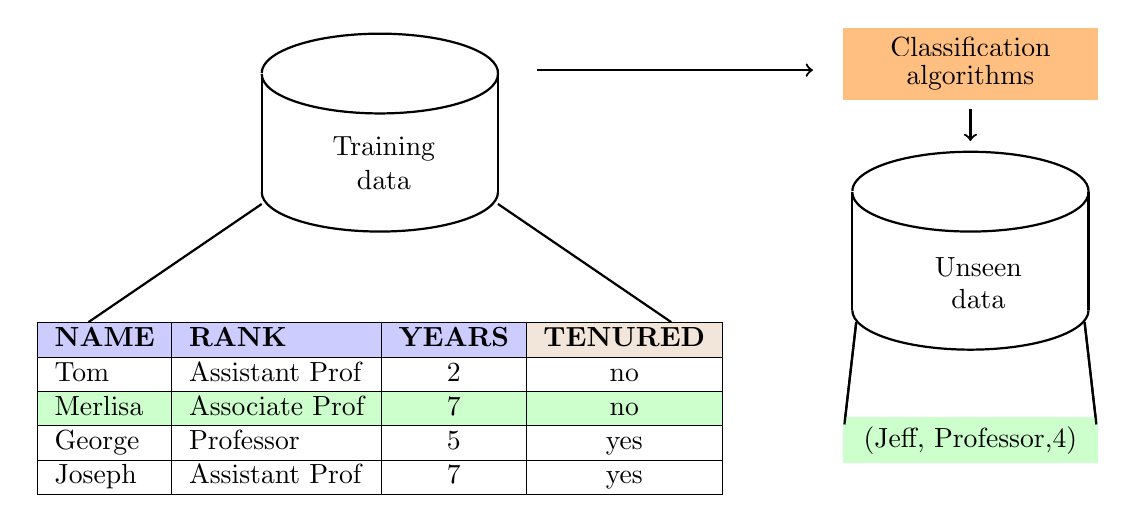
\begin{tikzpicture}
		\draw [thick](-1.5,3.15) -- (-1.5,4.65);
		\draw [thick](1.5,3.15) -- (1.5,4.65);
		\draw [thick](-1.5,3.15) arc (180:360:1.5 and 0.5);
		\draw [thick](-1.5,4.65) arc (180:360:1.5 and 0.5);
		\draw [thick](1.5,4.65) arc (-1.5:180:1.5 and 0.5);
		\draw [thick, ->] (2,4.7) -- (5.5,4.7);
		\draw [thick, ->] (7.5,4.2) -- (7.5,3.8);
		\draw [thick] (6.05,1.5) -- (5.9,0.2);
		\draw [thick] (8.95,1.5) -- (9.1,0.2);
		\node[text width = 3cm, align=center] at (0.05,3.7) {Training};
		\node[text width = 3cm, align=center] at (0.05,3.3) {data};

		\node[text width = 3cm, align=center] at (7.6,2.2) {Unseen};
		\node[text width = 3cm, align=center] at (7.6,1.8) {data};

		\node at (0,0.4){
			\begin{tabular}{|l|l|c|c|}
				\hline
				\cellcolor{blue!20}\textbf{\uppercase{name}} & \cellcolor{blue!20}\textbf{\uppercase{rank}} & \cellcolor{blue!20}\textbf{\uppercase{years}} & \cellcolor{brown!20}\textbf{\uppercase{tenured}} \\\hline
				Tom                                          & Assistant Prof                               & 2                                             & no                                               \\\hline
				\cellcolor{green!20}Merlisa                  & \cellcolor{green!20}Associate Prof           & \cellcolor{green!20}7                         & \cellcolor{green!20}no                           \\\hline
				George                                       & Professor                                    & 5                                             & yes                                              \\\hline
				Joseph                                       & Assistant Prof                               & 7                                             & yes                                              \\\hline
			\end{tabular}
		};
		\node[fill=orange!50, text width = 3cm, align=center] at (7.5,5) {Classification};
		\node[fill=orange!50, text width = 3cm, align=center] at (7.5,4.6) {algorithms};
		\node[fill=green!20, text width = 3cm, align=center] at (7.5,0) {(Jeff, Professor,4)};
		\draw [thick] (6.05,1.5) -- (5.9,0.2);
		\draw [thick] (8.95,1.5) -- (9.1,0.2);
		\draw [thick](6,1.65) -- (6,3.15);
		\draw [thick](9,1.65) -- (9,3.15);
		\draw [thick](6,1.65) arc (180:360:1.5 and 0.5);
		\draw [thick](6,3.15) arc (180:360:1.5 and 0.5);
		\draw [thick](9,3.15) arc (-1.5:180:1.5 and 0.5);
		\draw [thick] (-3.7,1.5) -- (-1.5,3);
		\draw [thick] (1.5,3) -- (3.7,1.5);
	\end{tikzpicture}
\end{frame}
